% Options for packages loaded elsewhere
% Options for packages loaded elsewhere
\PassOptionsToPackage{unicode}{hyperref}
\PassOptionsToPackage{hyphens}{url}
\PassOptionsToPackage{dvipsnames,svgnames,x11names}{xcolor}
%
\documentclass[
  letterpaper,
  DIV=11,
  numbers=noendperiod]{scrartcl}
\usepackage{xcolor}
\usepackage[top=30mm,left=30mm]{geometry}
\usepackage{amsmath,amssymb}
\setcounter{secnumdepth}{-\maxdimen} % remove section numbering
\usepackage{iftex}
\ifPDFTeX
  \usepackage[T1]{fontenc}
  \usepackage[utf8]{inputenc}
  \usepackage{textcomp} % provide euro and other symbols
\else % if luatex or xetex
  \usepackage{unicode-math} % this also loads fontspec
  \defaultfontfeatures{Scale=MatchLowercase}
  \defaultfontfeatures[\rmfamily]{Ligatures=TeX,Scale=1}
\fi
\usepackage{lmodern}
\ifPDFTeX\else
  % xetex/luatex font selection
\fi
% Use upquote if available, for straight quotes in verbatim environments
\IfFileExists{upquote.sty}{\usepackage{upquote}}{}
\IfFileExists{microtype.sty}{% use microtype if available
  \usepackage[]{microtype}
  \UseMicrotypeSet[protrusion]{basicmath} % disable protrusion for tt fonts
}{}
\makeatletter
\@ifundefined{KOMAClassName}{% if non-KOMA class
  \IfFileExists{parskip.sty}{%
    \usepackage{parskip}
  }{% else
    \setlength{\parindent}{0pt}
    \setlength{\parskip}{6pt plus 2pt minus 1pt}}
}{% if KOMA class
  \KOMAoptions{parskip=half}}
\makeatother
% Make \paragraph and \subparagraph free-standing
\makeatletter
\ifx\paragraph\undefined\else
  \let\oldparagraph\paragraph
  \renewcommand{\paragraph}{
    \@ifstar
      \xxxParagraphStar
      \xxxParagraphNoStar
  }
  \newcommand{\xxxParagraphStar}[1]{\oldparagraph*{#1}\mbox{}}
  \newcommand{\xxxParagraphNoStar}[1]{\oldparagraph{#1}\mbox{}}
\fi
\ifx\subparagraph\undefined\else
  \let\oldsubparagraph\subparagraph
  \renewcommand{\subparagraph}{
    \@ifstar
      \xxxSubParagraphStar
      \xxxSubParagraphNoStar
  }
  \newcommand{\xxxSubParagraphStar}[1]{\oldsubparagraph*{#1}\mbox{}}
  \newcommand{\xxxSubParagraphNoStar}[1]{\oldsubparagraph{#1}\mbox{}}
\fi
\makeatother

\usepackage{color}
\usepackage{fancyvrb}
\newcommand{\VerbBar}{|}
\newcommand{\VERB}{\Verb[commandchars=\\\{\}]}
\DefineVerbatimEnvironment{Highlighting}{Verbatim}{commandchars=\\\{\}}
% Add ',fontsize=\small' for more characters per line
\usepackage{framed}
\definecolor{shadecolor}{RGB}{241,243,245}
\newenvironment{Shaded}{\begin{snugshade}}{\end{snugshade}}
\newcommand{\AlertTok}[1]{\textcolor[rgb]{0.68,0.00,0.00}{#1}}
\newcommand{\AnnotationTok}[1]{\textcolor[rgb]{0.37,0.37,0.37}{#1}}
\newcommand{\AttributeTok}[1]{\textcolor[rgb]{0.40,0.45,0.13}{#1}}
\newcommand{\BaseNTok}[1]{\textcolor[rgb]{0.68,0.00,0.00}{#1}}
\newcommand{\BuiltInTok}[1]{\textcolor[rgb]{0.00,0.23,0.31}{#1}}
\newcommand{\CharTok}[1]{\textcolor[rgb]{0.13,0.47,0.30}{#1}}
\newcommand{\CommentTok}[1]{\textcolor[rgb]{0.37,0.37,0.37}{#1}}
\newcommand{\CommentVarTok}[1]{\textcolor[rgb]{0.37,0.37,0.37}{\textit{#1}}}
\newcommand{\ConstantTok}[1]{\textcolor[rgb]{0.56,0.35,0.01}{#1}}
\newcommand{\ControlFlowTok}[1]{\textcolor[rgb]{0.00,0.23,0.31}{\textbf{#1}}}
\newcommand{\DataTypeTok}[1]{\textcolor[rgb]{0.68,0.00,0.00}{#1}}
\newcommand{\DecValTok}[1]{\textcolor[rgb]{0.68,0.00,0.00}{#1}}
\newcommand{\DocumentationTok}[1]{\textcolor[rgb]{0.37,0.37,0.37}{\textit{#1}}}
\newcommand{\ErrorTok}[1]{\textcolor[rgb]{0.68,0.00,0.00}{#1}}
\newcommand{\ExtensionTok}[1]{\textcolor[rgb]{0.00,0.23,0.31}{#1}}
\newcommand{\FloatTok}[1]{\textcolor[rgb]{0.68,0.00,0.00}{#1}}
\newcommand{\FunctionTok}[1]{\textcolor[rgb]{0.28,0.35,0.67}{#1}}
\newcommand{\ImportTok}[1]{\textcolor[rgb]{0.00,0.46,0.62}{#1}}
\newcommand{\InformationTok}[1]{\textcolor[rgb]{0.37,0.37,0.37}{#1}}
\newcommand{\KeywordTok}[1]{\textcolor[rgb]{0.00,0.23,0.31}{\textbf{#1}}}
\newcommand{\NormalTok}[1]{\textcolor[rgb]{0.00,0.23,0.31}{#1}}
\newcommand{\OperatorTok}[1]{\textcolor[rgb]{0.37,0.37,0.37}{#1}}
\newcommand{\OtherTok}[1]{\textcolor[rgb]{0.00,0.23,0.31}{#1}}
\newcommand{\PreprocessorTok}[1]{\textcolor[rgb]{0.68,0.00,0.00}{#1}}
\newcommand{\RegionMarkerTok}[1]{\textcolor[rgb]{0.00,0.23,0.31}{#1}}
\newcommand{\SpecialCharTok}[1]{\textcolor[rgb]{0.37,0.37,0.37}{#1}}
\newcommand{\SpecialStringTok}[1]{\textcolor[rgb]{0.13,0.47,0.30}{#1}}
\newcommand{\StringTok}[1]{\textcolor[rgb]{0.13,0.47,0.30}{#1}}
\newcommand{\VariableTok}[1]{\textcolor[rgb]{0.07,0.07,0.07}{#1}}
\newcommand{\VerbatimStringTok}[1]{\textcolor[rgb]{0.13,0.47,0.30}{#1}}
\newcommand{\WarningTok}[1]{\textcolor[rgb]{0.37,0.37,0.37}{\textit{#1}}}

\usepackage{longtable,booktabs,array}
\newcounter{none} % for unnumbered tables
\usepackage{calc} % for calculating minipage widths
% Correct order of tables after \paragraph or \subparagraph
\usepackage{etoolbox}
\makeatletter
\patchcmd\longtable{\par}{\if@noskipsec\mbox{}\fi\par}{}{}
\makeatother
% Allow footnotes in longtable head/foot
\IfFileExists{footnotehyper.sty}{\usepackage{footnotehyper}}{\usepackage{footnote}}
\makesavenoteenv{longtable}
\usepackage{graphicx}
\makeatletter
\newsavebox\pandoc@box
\newcommand*\pandocbounded[1]{% scales image to fit in text height/width
  \sbox\pandoc@box{#1}%
  \Gscale@div\@tempa{\textheight}{\dimexpr\ht\pandoc@box+\dp\pandoc@box\relax}%
  \Gscale@div\@tempb{\linewidth}{\wd\pandoc@box}%
  \ifdim\@tempb\p@<\@tempa\p@\let\@tempa\@tempb\fi% select the smaller of both
  \ifdim\@tempa\p@<\p@\scalebox{\@tempa}{\usebox\pandoc@box}%
  \else\usebox{\pandoc@box}%
  \fi%
}
% Set default figure placement to htbp
\def\fps@figure{htbp}
\makeatother





\setlength{\emergencystretch}{3em} % prevent overfull lines

\providecommand{\tightlist}{%
  \setlength{\itemsep}{0pt}\setlength{\parskip}{0pt}}



 


\KOMAoption{captions}{tableheading}
\makeatletter
\@ifpackageloaded{caption}{}{\usepackage{caption}}
\AtBeginDocument{%
\ifdefined\contentsname
  \renewcommand*\contentsname{Table of contents}
\else
  \newcommand\contentsname{Table of contents}
\fi
\ifdefined\listfigurename
  \renewcommand*\listfigurename{List of Figures}
\else
  \newcommand\listfigurename{List of Figures}
\fi
\ifdefined\listtablename
  \renewcommand*\listtablename{List of Tables}
\else
  \newcommand\listtablename{List of Tables}
\fi
\ifdefined\figurename
  \renewcommand*\figurename{Figure}
\else
  \newcommand\figurename{Figure}
\fi
\ifdefined\tablename
  \renewcommand*\tablename{Table}
\else
  \newcommand\tablename{Table}
\fi
}
\@ifpackageloaded{float}{}{\usepackage{float}}
\floatstyle{ruled}
\@ifundefined{c@chapter}{\newfloat{codelisting}{h}{lop}}{\newfloat{codelisting}{h}{lop}[chapter]}
\floatname{codelisting}{Listing}
\newcommand*\listoflistings{\listof{codelisting}{List of Listings}}
\makeatother
\makeatletter
\makeatother
\makeatletter
\@ifpackageloaded{caption}{}{\usepackage{caption}}
\@ifpackageloaded{subcaption}{}{\usepackage{subcaption}}
\makeatother
\usepackage{bookmark}
\IfFileExists{xurl.sty}{\usepackage{xurl}}{} % add URL line breaks if available
\urlstyle{same}
\hypersetup{
  pdftitle={deepSSF Data Prep - S2},
  pdfauthor={Scott Forrest},
  colorlinks=true,
  linkcolor={blue},
  filecolor={Maroon},
  citecolor={Blue},
  urlcolor={Blue},
  pdfcreator={LaTeX via pandoc}}


\title{deepSSF Data Prep - S2}
\author{Scott Forrest}
\date{2025-02-18}
\begin{document}
\maketitle
\begin{abstract}
This document outlines the steps taken to prepare the data for the
deepSSF model fitting, using Sentinel-2 data directly (instead of
derived covariates such as NDVI).
\end{abstract}

\renewcommand*\contentsname{Table of contents}
{
\setcounter{tocdepth}{3}
\tableofcontents
}

\subsection{Loading packages}\label{loading-packages}

\begin{Shaded}
\begin{Highlighting}[]
\FunctionTok{library}\NormalTok{(tidyverse)}
\NormalTok{packages }\OtherTok{\textless{}{-}} \FunctionTok{c}\NormalTok{(}\StringTok{"amt"}\NormalTok{, }\StringTok{"sf"}\NormalTok{, }\StringTok{"terra"}\NormalTok{, }\StringTok{"beepr"}\NormalTok{, }\StringTok{"tictoc"}\NormalTok{)}
\FunctionTok{walk}\NormalTok{(packages, require, }\AttributeTok{character.only =}\NormalTok{ T)}
\end{Highlighting}
\end{Shaded}

\subsection{Import data and clean}\label{import-data-and-clean}

\begin{Shaded}
\begin{Highlighting}[]
\NormalTok{buffalo }\OtherTok{\textless{}{-}} \FunctionTok{read\_csv}\NormalTok{(}\StringTok{"data/buffalo.csv"}\NormalTok{)}
\end{Highlighting}
\end{Shaded}

\begin{verbatim}
New names:
Rows: 133161 Columns: 11
-- Column specification
-------------------------------------------------------- Delimiter: "," chr
(2): node, dates dbl (7): ...1, lat, lon, height, accuracy, heading, speed dttm
(2): timestamp, DateTime
i Use `spec()` to retrieve the full column specification for this data. i
Specify the column types or set `show_col_types = FALSE` to quiet this message.
* `` -> `...1`
\end{verbatim}

\begin{Shaded}
\begin{Highlighting}[]
\CommentTok{\# remove individuals that have poor data quality or less than about 3 months of data. }
\CommentTok{\# The "2014.GPS\_COMPACT copy.csv" string is a duplicate of ID 2024, so we exlcude it}
\NormalTok{buffalo }\OtherTok{\textless{}{-}}\NormalTok{ buffalo }\SpecialCharTok{\%\textgreater{}\%} \FunctionTok{filter}\NormalTok{(}\SpecialCharTok{!}\NormalTok{node }\SpecialCharTok{\%in\%} \FunctionTok{c}\NormalTok{(}\StringTok{"2014.GPS\_COMPACT copy.csv"}\NormalTok{, }
                                           \CommentTok{\# 2005, 2014, 2018, 2021, 2022, 2024,}
                                           \DecValTok{2029}\NormalTok{, }\DecValTok{2043}\NormalTok{, }\DecValTok{2265}\NormalTok{, }\DecValTok{2284}\NormalTok{, }\DecValTok{2346}\NormalTok{, }\DecValTok{2354}\NormalTok{))}

\NormalTok{buffalo }\OtherTok{\textless{}{-}}\NormalTok{ buffalo }\SpecialCharTok{\%\textgreater{}\%}  
  \FunctionTok{group\_by}\NormalTok{(node) }\SpecialCharTok{\%\textgreater{}\%} 
  \FunctionTok{arrange}\NormalTok{(DateTime, }\AttributeTok{.by\_group =}\NormalTok{ T) }\SpecialCharTok{\%\textgreater{}\%} 
  \FunctionTok{distinct}\NormalTok{(DateTime, }\AttributeTok{.keep\_all =}\NormalTok{ T) }\SpecialCharTok{\%\textgreater{}\%} 
  \FunctionTok{arrange}\NormalTok{(node) }\SpecialCharTok{\%\textgreater{}\%} 
  \FunctionTok{mutate}\NormalTok{(}\AttributeTok{ID =}\NormalTok{ node)}

\NormalTok{buffalo\_clean }\OtherTok{\textless{}{-}}\NormalTok{ buffalo[, }\FunctionTok{c}\NormalTok{(}\DecValTok{12}\NormalTok{, }\DecValTok{2}\NormalTok{, }\DecValTok{4}\NormalTok{, }\DecValTok{3}\NormalTok{)]}
\FunctionTok{colnames}\NormalTok{(buffalo\_clean) }\OtherTok{\textless{}{-}} \FunctionTok{c}\NormalTok{(}\StringTok{"id"}\NormalTok{, }\StringTok{"time"}\NormalTok{, }\StringTok{"lon"}\NormalTok{, }\StringTok{"lat"}\NormalTok{)}
\FunctionTok{attr}\NormalTok{(buffalo\_clean}\SpecialCharTok{$}\NormalTok{time, }\StringTok{"tzone"}\NormalTok{) }\OtherTok{\textless{}{-}} \StringTok{"Australia/Queensland"}
\FunctionTok{head}\NormalTok{(buffalo\_clean)}
\end{Highlighting}
\end{Shaded}

\begin{verbatim}
# A tibble: 6 x 4
  id    time                  lon   lat
  <chr> <dttm>              <dbl> <dbl>
1 2005  2018-07-25 10:04:02  134. -12.3
2 2005  2018-07-25 11:04:23  134. -12.3
3 2005  2018-07-25 12:04:39  134. -12.3
4 2005  2018-07-25 13:04:17  134. -12.3
5 2005  2018-07-25 14:04:39  134. -12.3
6 2005  2018-07-25 15:04:27  134. -12.3
\end{verbatim}

\begin{Shaded}
\begin{Highlighting}[]
\FunctionTok{tz}\NormalTok{(buffalo\_clean}\SpecialCharTok{$}\NormalTok{time)}
\end{Highlighting}
\end{Shaded}

\begin{verbatim}
[1] "Australia/Queensland"
\end{verbatim}

\begin{Shaded}
\begin{Highlighting}[]
\NormalTok{buffalo\_ids }\OtherTok{\textless{}{-}} \FunctionTok{unique}\NormalTok{(buffalo\_clean}\SpecialCharTok{$}\NormalTok{id)}
\end{Highlighting}
\end{Shaded}

\subsection{Setup trajectory}\label{setup-trajectory}

Use the \texttt{amt} package to create a trajectory object from the
cleaned data.

\begin{Shaded}
\begin{Highlighting}[]
\NormalTok{buffalo\_all }\OtherTok{\textless{}{-}}\NormalTok{ buffalo\_clean }\SpecialCharTok{\%\textgreater{}\%} \FunctionTok{mk\_track}\NormalTok{(}\AttributeTok{id =}\NormalTok{ id,}
\NormalTok{                                           lon,}
\NormalTok{                                           lat, }
\NormalTok{                                           time, }
                                           \AttributeTok{all\_cols =}\NormalTok{ T,}
                                           \AttributeTok{crs =} \DecValTok{4326}\NormalTok{) }\SpecialCharTok{\%\textgreater{}\%} 
  \FunctionTok{transform\_coords}\NormalTok{(}\AttributeTok{crs\_to =} \DecValTok{3112}\NormalTok{, }\AttributeTok{crs\_from =} \DecValTok{4326}\NormalTok{) }\CommentTok{\# Transformation to GDA94 / }
\CommentTok{\# Geoscience Australia Lambert (https://epsg.io/3112)}
\end{Highlighting}
\end{Shaded}

\subsection{Plot the data coloured by
time}\label{plot-the-data-coloured-by-time}

\begin{Shaded}
\begin{Highlighting}[]
\NormalTok{buffalo\_all }\SpecialCharTok{\%\textgreater{}\%}
  \FunctionTok{ggplot}\NormalTok{(}\FunctionTok{aes}\NormalTok{(}\AttributeTok{x =}\NormalTok{ x\_, }\AttributeTok{y =}\NormalTok{ y\_, }\AttributeTok{colour =}\NormalTok{ t\_)) }\SpecialCharTok{+}
  \FunctionTok{geom\_point}\NormalTok{(}\AttributeTok{alpha =} \FloatTok{0.25}\NormalTok{, }\AttributeTok{size =} \DecValTok{1}\NormalTok{) }\SpecialCharTok{+} 
  \FunctionTok{coord\_fixed}\NormalTok{() }\SpecialCharTok{+}
  \FunctionTok{scale\_colour\_viridis\_c}\NormalTok{() }\SpecialCharTok{+}
  \FunctionTok{theme\_classic}\NormalTok{()}
\end{Highlighting}
\end{Shaded}

\pandocbounded{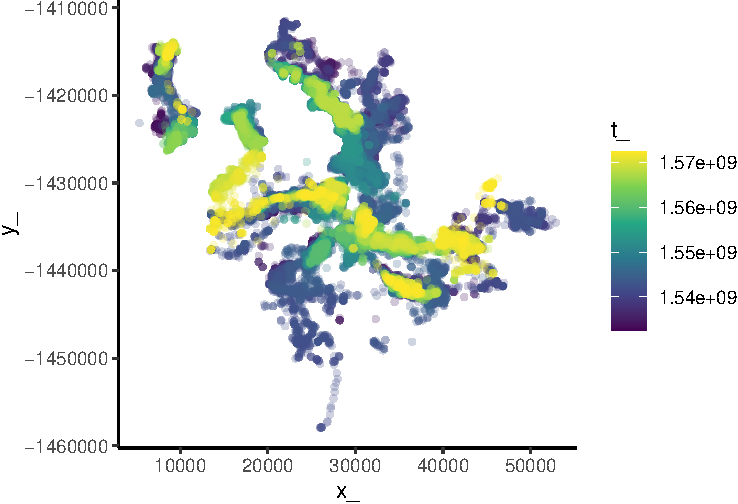
\includegraphics[keepaspectratio]{deepSSF_data_prep_S2_id_files/figure-pdf/unnamed-chunk-4-1.pdf}}

\subsection{Reading in the environmental
covariates}\label{reading-in-the-environmental-covariates}

\begin{Shaded}
\begin{Highlighting}[]
\NormalTok{slope }\OtherTok{\textless{}{-}} \FunctionTok{rast}\NormalTok{(}\StringTok{"mapping/cropped rasters/slope\_raster.tif"}\NormalTok{)}
\FunctionTok{names}\NormalTok{(slope) }\OtherTok{\textless{}{-}} \StringTok{"slope"}
\FunctionTok{plot}\NormalTok{(slope)}
\end{Highlighting}
\end{Shaded}

\pandocbounded{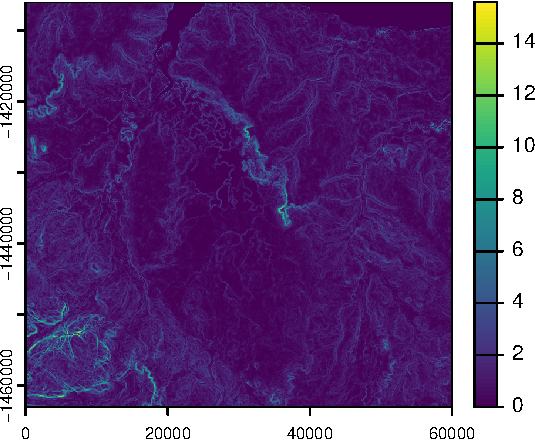
\includegraphics[keepaspectratio]{deepSSF_data_prep_S2_id_files/figure-pdf/unnamed-chunk-5-1.pdf}}

\subsection{Sentinel-2 spectral
layers}\label{sentinel-2-spectral-layers}

Create vector of dates. We just use the 15th of the month (the layers
were averaged across the month).

\begin{Shaded}
\begin{Highlighting}[]
\NormalTok{dates }\OtherTok{\textless{}{-}} \FunctionTok{as.POSIXct}\NormalTok{(lubridate}\SpecialCharTok{::}\FunctionTok{ymd}\NormalTok{(}\StringTok{"2019{-}01{-}15"}\NormalTok{)) }\SpecialCharTok{+} \FunctionTok{months}\NormalTok{(}\DecValTok{0}\SpecialCharTok{:}\DecValTok{11}\NormalTok{)}
\end{Highlighting}
\end{Shaded}

\subsubsection{Import the layers and add
times}\label{import-the-layers-and-add-times}

Each of these stacks are one month of the 12 bands of Sentinel-2 data.
Initially they are at 10m resolution, but we resample them to 25m to
match the resolution of the slope layer.

We save each of the scaled rasters such that we can import them when we
simulate from the deepSSF model using the Sentinel-2 data.

As the resampling takes some time, we have commented this code out and
read in the resampled and scaled layers direclty in the next code chunk.

\begin{Shaded}
\begin{Highlighting}[]
\CommentTok{\# }\AlertTok{\#\#\#}\CommentTok{ January 2019}
\CommentTok{\# s2\_10m\_2019\_01 \textless{}{-} rast("mapping/cropped rasters/sentinel2/10m/S2\_SR\_masked\_2019\_01.tif")}
\CommentTok{\# terra::time(s2\_10m\_2019\_01) \textless{}{-} rep(as.POSIXct(lubridate::ymd("2019{-}01{-}15"), }
\CommentTok{\#                                               tz = "Australia/Queensland"), }
\CommentTok{\#                                    nlyr(s2\_10m\_2019\_01))}
\CommentTok{\# s2\_25m\_2019\_01 \textless{}{-} terra::resample(s2\_10m\_2019\_01, slope, method = "bilinear")}
\CommentTok{\# s2\_25m\_2019\_01 \textless{}{-} s2\_25m\_2019\_01 / 10000}
\CommentTok{\# \# to save the scaled raster to file for reading when simulating from the deepSSF model}
\CommentTok{\# \# writeRaster(s2\_25m\_2019\_01, "mapping/cropped rasters/sentinel2/25m/S2\_SR\_masked\_scaled\_25m\_2019\_01.tif", overwrite = T)}
\CommentTok{\# }
\CommentTok{\# }
\CommentTok{\# }\AlertTok{\#\#\#}\CommentTok{ February 2019}
\CommentTok{\# s2\_10m\_2019\_02 \textless{}{-} rast("mapping/cropped rasters/sentinel2/10m/S2\_SR\_masked\_2019\_02.tif")}
\CommentTok{\# terra::time(s2\_10m\_2019\_02) \textless{}{-} rep(as.POSIXct(lubridate::ymd("2019{-}02{-}15"), }
\CommentTok{\#                                               tz = "Australia/Queensland"), }
\CommentTok{\#                                    nlyr(s2\_10m\_2019\_02))}
\CommentTok{\# s2\_25m\_2019\_02 \textless{}{-} terra::resample(s2\_10m\_2019\_02, slope, method = "bilinear")}
\CommentTok{\# s2\_25m\_2019\_02 \textless{}{-} s2\_25m\_2019\_02 / 10000}
\CommentTok{\# \# writeRaster(s2\_25m\_2019\_02, "mapping/cropped rasters/sentinel2/25m/S2\_SR\_masked\_scaled\_25m\_2019\_02.tif", overwrite = T)}
\CommentTok{\# }
\CommentTok{\# }\AlertTok{\#\#\#}\CommentTok{ March 2019}
\CommentTok{\# s2\_10m\_2019\_03 \textless{}{-} rast("mapping/cropped rasters/sentinel2/10m/S2\_SR\_masked\_2019\_03.tif")}
\CommentTok{\# terra::time(s2\_10m\_2019\_03) \textless{}{-} rep(as.POSIXct(lubridate::ymd("2019{-}03{-}15"), }
\CommentTok{\#                                               tz = "Australia/Queensland"), }
\CommentTok{\#                                    nlyr(s2\_10m\_2019\_03))}
\CommentTok{\# s2\_25m\_2019\_03 \textless{}{-} terra::resample(s2\_10m\_2019\_03, slope, method = "bilinear")}
\CommentTok{\# s2\_25m\_2019\_03 \textless{}{-} s2\_25m\_2019\_03 / 10000}
\CommentTok{\# \# writeRaster(s2\_25m\_2019\_03, "mapping/cropped rasters/sentinel2/25m/S2\_SR\_masked\_scaled\_25m\_2019\_03.tif", overwrite = T)}
\CommentTok{\# }
\CommentTok{\# }\AlertTok{\#\#\#}\CommentTok{ April 2019}
\CommentTok{\# s2\_10m\_2019\_04 \textless{}{-} rast("mapping/cropped rasters/sentinel2/10m/S2\_SR\_masked\_2019\_04.tif")}
\CommentTok{\# terra::time(s2\_10m\_2019\_04) \textless{}{-} rep(as.POSIXct(lubridate::ymd("2019{-}04{-}15"), }
\CommentTok{\#                                               tz = "Australia/Queensland"), }
\CommentTok{\#                                    nlyr(s2\_10m\_2019\_04))}
\CommentTok{\# s2\_25m\_2019\_04 \textless{}{-} terra::resample(s2\_10m\_2019\_04, slope, method = "bilinear")}
\CommentTok{\# s2\_25m\_2019\_04 \textless{}{-} s2\_25m\_2019\_04 / 10000}
\CommentTok{\# \# writeRaster(s2\_25m\_2019\_04, "mapping/cropped rasters/sentinel2/25m/S2\_SR\_masked\_scaled\_25m\_2019\_04.tif", overwrite = T)}
\CommentTok{\# }
\CommentTok{\# }
\CommentTok{\# }\AlertTok{\#\#\#}\CommentTok{ May 2019}
\CommentTok{\# s2\_10m\_2019\_05 \textless{}{-} rast("mapping/cropped rasters/sentinel2/10m/S2\_SR\_masked\_2019\_05.tif")}
\CommentTok{\# terra::time(s2\_10m\_2019\_05) \textless{}{-} rep(as.POSIXct(lubridate::ymd("2019{-}05{-}15"), }
\CommentTok{\#                                               tz = "Australia/Queensland"), }
\CommentTok{\#                                    nlyr(s2\_10m\_2019\_05))}
\CommentTok{\# s2\_25m\_2019\_05 \textless{}{-} terra::resample(s2\_10m\_2019\_05, slope, method = "bilinear")}
\CommentTok{\# s2\_25m\_2019\_05 \textless{}{-} s2\_25m\_2019\_05 / 10000}
\CommentTok{\# \# writeRaster(s2\_25m\_2019\_05, "mapping/cropped rasters/sentinel2/25m/S2\_SR\_masked\_scaled\_25m\_2019\_05.tif", overwrite = T)}
\CommentTok{\# }
\CommentTok{\# }\AlertTok{\#\#\#}\CommentTok{ June 2019}
\CommentTok{\# s2\_10m\_2019\_06 \textless{}{-} rast("mapping/cropped rasters/sentinel2/10m/S2\_SR\_masked\_2019\_06.tif")}
\CommentTok{\# \# plot(s2\_10m\_2019\_06[[2]])}
\CommentTok{\# terra::time(s2\_10m\_2019\_06) \textless{}{-} rep(as.POSIXct(lubridate::ymd("2019{-}06{-}15"), }
\CommentTok{\#                                               tz = "Australia/Queensland"), }
\CommentTok{\#                                    nlyr(s2\_10m\_2019\_06))}
\CommentTok{\# s2\_25m\_2019\_06 \textless{}{-} terra::resample(s2\_10m\_2019\_06, slope, method = "bilinear")}
\CommentTok{\# s2\_25m\_2019\_06 \textless{}{-} s2\_25m\_2019\_06 / 10000}
\CommentTok{\# \# writeRaster(s2\_25m\_2019\_06, "mapping/cropped rasters/sentinel2/25m/S2\_SR\_masked\_scaled\_25m\_2019\_06.tif", overwrite = T)}
\CommentTok{\# }
\CommentTok{\# }\AlertTok{\#\#\#}\CommentTok{ July 2019}
\CommentTok{\# s2\_10m\_2019\_07 \textless{}{-} rast("mapping/cropped rasters/sentinel2/10m/S2\_SR\_masked\_2019\_07.tif")}
\CommentTok{\# terra::time(s2\_10m\_2019\_07) \textless{}{-} rep(as.POSIXct(lubridate::ymd("2019{-}07{-}15"), }
\CommentTok{\#                                               tz = "Australia/Queensland"), }
\CommentTok{\#                                    nlyr(s2\_10m\_2019\_07))}
\CommentTok{\# s2\_25m\_2019\_07 \textless{}{-} terra::resample(s2\_10m\_2019\_07, slope, method = "bilinear")}
\CommentTok{\# s2\_25m\_2019\_07 \textless{}{-} s2\_25m\_2019\_07 / 10000}
\CommentTok{\# \# writeRaster(s2\_25m\_2019\_07, "mapping/cropped rasters/sentinel2/25m/S2\_SR\_masked\_scaled\_25m\_2019\_07.tif", overwrite = T)}
\CommentTok{\# }
\CommentTok{\# }\AlertTok{\#\#\#}\CommentTok{ August 2019}
\CommentTok{\# s2\_10m\_2019\_08 \textless{}{-} rast("mapping/cropped rasters/sentinel2/10m/S2\_SR\_masked\_2019\_08.tif")}
\CommentTok{\# terra::time(s2\_10m\_2019\_08) \textless{}{-} rep(as.POSIXct(lubridate::ymd("2019{-}08{-}15"), }
\CommentTok{\#                                               tz = "Australia/Queensland"), }
\CommentTok{\#                                    nlyr(s2\_10m\_2019\_08))}
\CommentTok{\# s2\_25m\_2019\_08 \textless{}{-} terra::resample(s2\_10m\_2019\_08, slope, method = "bilinear")}
\CommentTok{\# s2\_25m\_2019\_08 \textless{}{-} s2\_25m\_2019\_08 / 10000}
\CommentTok{\# \# writeRaster(s2\_25m\_2019\_08, "mapping/cropped rasters/sentinel2/25m/S2\_SR\_masked\_scaled\_25m\_2019\_08.tif", overwrite = T)}
\CommentTok{\# }
\CommentTok{\# }\AlertTok{\#\#\#}\CommentTok{ September 2019}
\CommentTok{\# s2\_10m\_2019\_09 \textless{}{-} rast("mapping/cropped rasters/sentinel2/10m/S2\_SR\_masked\_2019\_09.tif")}
\CommentTok{\# terra::time(s2\_10m\_2019\_09) \textless{}{-} rep(as.POSIXct(lubridate::ymd("2019{-}09{-}15"), }
\CommentTok{\#                                               tz = "Australia/Queensland"), }
\CommentTok{\#                                    nlyr(s2\_10m\_2019\_09))}
\CommentTok{\# s2\_25m\_2019\_09 \textless{}{-} terra::resample(s2\_10m\_2019\_09, slope, method = "bilinear")}
\CommentTok{\# s2\_25m\_2019\_09 \textless{}{-} s2\_25m\_2019\_09 / 10000}
\CommentTok{\# \# writeRaster(s2\_25m\_2019\_09, "mapping/cropped rasters/sentinel2/25m/S2\_SR\_masked\_scaled\_25m\_2019\_09.tif", overwrite = T)}
\CommentTok{\# }
\CommentTok{\# }\AlertTok{\#\#\#}\CommentTok{ October 2019}
\CommentTok{\# s2\_10m\_2019\_10 \textless{}{-} rast("mapping/cropped rasters/sentinel2/10m/S2\_SR\_masked\_2019\_10.tif")}
\CommentTok{\# terra::time(s2\_10m\_2019\_10) \textless{}{-} rep(as.POSIXct(lubridate::ymd("2019{-}10{-}15"), }
\CommentTok{\#                                               tz = "Australia/Queensland"), }
\CommentTok{\#                                    nlyr(s2\_10m\_2019\_10))}
\CommentTok{\# s2\_25m\_2019\_10 \textless{}{-} terra::resample(s2\_10m\_2019\_10, slope, method = "bilinear")}
\CommentTok{\# s2\_25m\_2019\_10 \textless{}{-} s2\_25m\_2019\_10 / 10000}
\CommentTok{\# \# writeRaster(s2\_25m\_2019\_10, "mapping/cropped rasters/sentinel2/25m/S2\_SR\_masked\_scaled\_25m\_2019\_10.tif", overwrite = T)}
\CommentTok{\# }
\CommentTok{\# }\AlertTok{\#\#\#}\CommentTok{ November 2019}
\CommentTok{\# s2\_10m\_2019\_11 \textless{}{-} rast("mapping/cropped rasters/sentinel2/10m/S2\_SR\_masked\_2019\_11.tif")}
\CommentTok{\# terra::time(s2\_10m\_2019\_11) \textless{}{-} rep(as.POSIXct(lubridate::ymd("2019{-}11{-}15"), }
\CommentTok{\#                                               tz = "Australia/Queensland"), }
\CommentTok{\#                                    nlyr(s2\_10m\_2019\_11))}
\CommentTok{\# s2\_25m\_2019\_11 \textless{}{-} terra::resample(s2\_10m\_2019\_11, slope, method = "bilinear")}
\CommentTok{\# s2\_25m\_2019\_11 \textless{}{-} s2\_25m\_2019\_11 / 10000}
\CommentTok{\# \# writeRaster(s2\_25m\_2019\_11, "mapping/cropped rasters/sentinel2/25m/S2\_SR\_masked\_scaled\_25m\_2019\_11.tif", overwrite = T)}
\CommentTok{\# }
\CommentTok{\# }\AlertTok{\#\#\#}\CommentTok{ December 2019}
\CommentTok{\# s2\_10m\_2019\_12 \textless{}{-} rast("mapping/cropped rasters/sentinel2/10m/S2\_SR\_masked\_2019\_12.tif")}
\CommentTok{\# terra::time(s2\_10m\_2019\_12) \textless{}{-} rep(as.POSIXct(lubridate::ymd("2019{-}12{-}15"), }
\CommentTok{\#                                               tz = "Australia/Queensland"), }
\CommentTok{\#                                    nlyr(s2\_10m\_2019\_12))}
\CommentTok{\# s2\_25m\_2019\_12 \textless{}{-} terra::resample(s2\_10m\_2019\_12, slope, method = "bilinear")}
\CommentTok{\# s2\_25m\_2019\_12 \textless{}{-} s2\_25m\_2019\_12 / 10000}
\CommentTok{\# \# writeRaster(s2\_25m\_2019\_12, "mapping/cropped rasters/sentinel2/25m/S2\_SR\_masked\_scaled\_25m\_2019\_12.tif", overwrite = T)}
\end{Highlighting}
\end{Shaded}

Each raster stack contains the Sentinel 2 bands for a given month in
2019, and have been scaled by 10,000 from what was downloaded from GEE.

\begin{Shaded}
\begin{Highlighting}[]
\NormalTok{s2\_25m\_2019\_01 }\OtherTok{\textless{}{-}} \FunctionTok{rast}\NormalTok{(}\StringTok{"mapping/cropped rasters/sentinel2/25m/S2\_SR\_masked\_scaled\_25m\_2019\_01.tif"}\NormalTok{)}
\NormalTok{s2\_25m\_2019\_02 }\OtherTok{\textless{}{-}} \FunctionTok{rast}\NormalTok{(}\StringTok{"mapping/cropped rasters/sentinel2/25m/S2\_SR\_masked\_scaled\_25m\_2019\_02.tif"}\NormalTok{)}
\NormalTok{s2\_25m\_2019\_03 }\OtherTok{\textless{}{-}} \FunctionTok{rast}\NormalTok{(}\StringTok{"mapping/cropped rasters/sentinel2/25m/S2\_SR\_masked\_scaled\_25m\_2019\_03.tif"}\NormalTok{)}
\NormalTok{s2\_25m\_2019\_04 }\OtherTok{\textless{}{-}} \FunctionTok{rast}\NormalTok{(}\StringTok{"mapping/cropped rasters/sentinel2/25m/S2\_SR\_masked\_scaled\_25m\_2019\_04.tif"}\NormalTok{)}
\NormalTok{s2\_25m\_2019\_05 }\OtherTok{\textless{}{-}} \FunctionTok{rast}\NormalTok{(}\StringTok{"mapping/cropped rasters/sentinel2/25m/S2\_SR\_masked\_scaled\_25m\_2019\_05.tif"}\NormalTok{)}
\NormalTok{s2\_25m\_2019\_06 }\OtherTok{\textless{}{-}} \FunctionTok{rast}\NormalTok{(}\StringTok{"mapping/cropped rasters/sentinel2/25m/S2\_SR\_masked\_scaled\_25m\_2019\_06.tif"}\NormalTok{)}
\NormalTok{s2\_25m\_2019\_07 }\OtherTok{\textless{}{-}} \FunctionTok{rast}\NormalTok{(}\StringTok{"mapping/cropped rasters/sentinel2/25m/S2\_SR\_masked\_scaled\_25m\_2019\_07.tif"}\NormalTok{)}
\NormalTok{s2\_25m\_2019\_08 }\OtherTok{\textless{}{-}} \FunctionTok{rast}\NormalTok{(}\StringTok{"mapping/cropped rasters/sentinel2/25m/S2\_SR\_masked\_scaled\_25m\_2019\_08.tif"}\NormalTok{)}
\NormalTok{s2\_25m\_2019\_09 }\OtherTok{\textless{}{-}} \FunctionTok{rast}\NormalTok{(}\StringTok{"mapping/cropped rasters/sentinel2/25m/S2\_SR\_masked\_scaled\_25m\_2019\_09.tif"}\NormalTok{)}
\NormalTok{s2\_25m\_2019\_10 }\OtherTok{\textless{}{-}} \FunctionTok{rast}\NormalTok{(}\StringTok{"mapping/cropped rasters/sentinel2/25m/S2\_SR\_masked\_scaled\_25m\_2019\_10.tif"}\NormalTok{)}
\NormalTok{s2\_25m\_2019\_11 }\OtherTok{\textless{}{-}} \FunctionTok{rast}\NormalTok{(}\StringTok{"mapping/cropped rasters/sentinel2/25m/S2\_SR\_masked\_scaled\_25m\_2019\_11.tif"}\NormalTok{)}
\NormalTok{s2\_25m\_2019\_12 }\OtherTok{\textless{}{-}} \FunctionTok{rast}\NormalTok{(}\StringTok{"mapping/cropped rasters/sentinel2/25m/S2\_SR\_masked\_scaled\_25m\_2019\_12.tif"}\NormalTok{)}

\NormalTok{s2\_25m\_2019\_01}
\end{Highlighting}
\end{Shaded}

\begin{verbatim}
class       : SpatRaster 
dimensions  : 2280, 2400, 12  (nrow, ncol, nlyr)
resolution  : 25, 25  (x, y)
extent      : 0, 60000, -1463000, -1406000  (xmin, xmax, ymin, ymax)
coord. ref. : GDA94 / Geoscience Australia Lambert (EPSG:3112) 
source      : S2_SR_masked_scaled_25m_2019_01.tif 
names       :       B1,         B2,         B3,        B4,         B5,         B6, ... 
min values  : 0.002600, 0.00298288, 0.01064496, 0.0101952, 0.01207968, 0.01042128, ... 
max values  : 0.313051, 0.40625551, 0.48839232, 0.5488096, 0.58363509, 0.57049966, ... 
time        : 2019-01-15 UTC 
\end{verbatim}

\subsubsection{Combine into a list}\label{combine-into-a-list}

\begin{Shaded}
\begin{Highlighting}[]
\NormalTok{s2\_list }\OtherTok{\textless{}{-}} \FunctionTok{list}\NormalTok{(s2\_25m\_2019\_01, }
\NormalTok{                s2\_25m\_2019\_02, }
\NormalTok{                s2\_25m\_2019\_03, }
\NormalTok{                s2\_25m\_2019\_04, }
\NormalTok{                s2\_25m\_2019\_05, }
\NormalTok{                s2\_25m\_2019\_06, }
\NormalTok{                s2\_25m\_2019\_07, }
\NormalTok{                s2\_25m\_2019\_08, }
\NormalTok{                s2\_25m\_2019\_09, }
\NormalTok{                s2\_25m\_2019\_10, }
\NormalTok{                s2\_25m\_2019\_11, }
\NormalTok{                s2\_25m\_2019\_12)}

\FunctionTok{names}\NormalTok{(s2\_25m\_2019\_12)}
\end{Highlighting}
\end{Shaded}

\begin{verbatim}
 [1] "B1"  "B2"  "B3"  "B4"  "B5"  "B6"  "B7"  "B8"  "B8A" "B9"  "B11" "B12"
\end{verbatim}

\section{Generating the data to fit a deepSSF
model}\label{generating-the-data-to-fit-a-deepssf-model}

\subsection{Set up the spatial extent of the local
covariates}\label{set-up-the-spatial-extent-of-the-local-covariates}

\begin{Shaded}
\begin{Highlighting}[]
\NormalTok{buffalo\_all }\OtherTok{\textless{}{-}}\NormalTok{ buffalo\_all }\SpecialCharTok{\%\textgreater{}\%}  
  \FunctionTok{arrange}\NormalTok{(id, t\_)}

\CommentTok{\# create a vector of ids}
\NormalTok{buffalo\_ids }\OtherTok{\textless{}{-}} \FunctionTok{unique}\NormalTok{(buffalo\_all}\SpecialCharTok{$}\NormalTok{id)}

\CommentTok{\# get the resolution from the covariates}
\NormalTok{res }\OtherTok{\textless{}{-}}\NormalTok{ terra}\SpecialCharTok{::}\FunctionTok{res}\NormalTok{(slope)[}\DecValTok{1}\NormalTok{]}

\CommentTok{\# how much to trim on either side of the location, }
\CommentTok{\# this will determine the extent of the spatial inputs to the deepSSF model}
\NormalTok{buffer }\OtherTok{\textless{}{-}} \DecValTok{1250} \SpecialCharTok{+}\NormalTok{ (res}\SpecialCharTok{/}\DecValTok{2}\NormalTok{)}
\CommentTok{\# calculate the number of cells in each axis}
\NormalTok{nxn\_cells }\OtherTok{\textless{}{-}}\NormalTok{ buffer}\SpecialCharTok{*}\DecValTok{2}\SpecialCharTok{/}\NormalTok{res}

\CommentTok{\# hourly lag {-} to set larger time differences between locations}
\NormalTok{hourly\_lag }\OtherTok{\textless{}{-}} \DecValTok{1}
\end{Highlighting}
\end{Shaded}

Loop over each individual and save the local rasters

\begin{Shaded}
\begin{Highlighting}[]
\ControlFlowTok{for}\NormalTok{(i }\ControlFlowTok{in} \DecValTok{1}\SpecialCharTok{:}\FunctionTok{length}\NormalTok{(buffalo\_ids)) \{}

\NormalTok{  buffalo\_data }\OtherTok{\textless{}{-}}\NormalTok{ buffalo\_all }\SpecialCharTok{\%\textgreater{}\%} \FunctionTok{filter}\NormalTok{(id }\SpecialCharTok{==}\NormalTok{ buffalo\_ids[i])}
  \CommentTok{\# all data for that individual}
  \CommentTok{\# buffalo\_data \textless{}{-} buffalo\_data \%\textgreater{}\% arrange(t\_)}
  \CommentTok{\# a subset of the data for that individual {-} mostly for testing}
\NormalTok{  buffalo\_data }\OtherTok{\textless{}{-}}\NormalTok{ buffalo\_data }\SpecialCharTok{\%\textgreater{}\%} \FunctionTok{arrange}\NormalTok{(t\_) }\SpecialCharTok{\%\textgreater{}\%} \FunctionTok{slice}\NormalTok{(}\DecValTok{1}\SpecialCharTok{:}\DecValTok{10}\NormalTok{)}
  
\NormalTok{  n\_samples }\OtherTok{\textless{}{-}} \FunctionTok{nrow}\NormalTok{(buffalo\_data)}
  
  \FunctionTok{tic}\NormalTok{()}
  
\NormalTok{  buffalo\_data\_covs }\OtherTok{\textless{}{-}}\NormalTok{ buffalo\_data }\SpecialCharTok{\%\textgreater{}\%} \FunctionTok{mutate}\NormalTok{(}
    
    \AttributeTok{x1\_ =}\NormalTok{ x\_,}
    \AttributeTok{y1\_ =}\NormalTok{ y\_,}
    \AttributeTok{x2\_ =} \FunctionTok{lead}\NormalTok{(x1\_, }\AttributeTok{n =}\NormalTok{ hourly\_lag, }\AttributeTok{default =} \ConstantTok{NA}\NormalTok{),}
    \AttributeTok{y2\_ =} \FunctionTok{lead}\NormalTok{(y1\_, }\AttributeTok{n =}\NormalTok{ hourly\_lag, }\AttributeTok{default =} \ConstantTok{NA}\NormalTok{),}
    \AttributeTok{x2\_cent =}\NormalTok{ x2\_ }\SpecialCharTok{{-}}\NormalTok{ x1\_,}
    \AttributeTok{y2\_cent =}\NormalTok{ y2\_ }\SpecialCharTok{{-}}\NormalTok{ y1\_,}
    \AttributeTok{t2\_ =} \FunctionTok{lead}\NormalTok{(t\_, }\AttributeTok{n =}\NormalTok{ hourly\_lag, }\AttributeTok{default =} \ConstantTok{NA}\NormalTok{),}
    \AttributeTok{t\_diff =} \FunctionTok{round}\NormalTok{(}\FunctionTok{difftime}\NormalTok{(t2\_, t\_, }\AttributeTok{units =} \StringTok{"hours"}\NormalTok{),}\DecValTok{0}\NormalTok{),}
    \AttributeTok{hour\_t1 =}\NormalTok{ lubridate}\SpecialCharTok{::}\FunctionTok{hour}\NormalTok{(t\_),}
    \AttributeTok{yday\_t1 =}\NormalTok{ lubridate}\SpecialCharTok{::}\FunctionTok{yday}\NormalTok{(t\_),}
    \AttributeTok{hour\_t2 =}\NormalTok{ lubridate}\SpecialCharTok{::}\FunctionTok{hour}\NormalTok{(t2\_),}
    \AttributeTok{hour\_t2\_sin =} \FunctionTok{sin}\NormalTok{(}\DecValTok{2}\SpecialCharTok{*}\NormalTok{pi}\SpecialCharTok{*}\NormalTok{hour\_t2}\SpecialCharTok{/}\DecValTok{24}\NormalTok{),}
    \AttributeTok{hour\_t2\_cos =} \FunctionTok{cos}\NormalTok{(}\DecValTok{2}\SpecialCharTok{*}\NormalTok{pi}\SpecialCharTok{*}\NormalTok{hour\_t2}\SpecialCharTok{/}\DecValTok{24}\NormalTok{),}
    \AttributeTok{yday\_t2 =}\NormalTok{ lubridate}\SpecialCharTok{::}\FunctionTok{yday}\NormalTok{(t2\_),}
    \AttributeTok{yday\_t2\_sin =} \FunctionTok{sin}\NormalTok{(}\DecValTok{2}\SpecialCharTok{*}\NormalTok{pi}\SpecialCharTok{*}\NormalTok{yday\_t2}\SpecialCharTok{/}\FloatTok{365.25}\NormalTok{),}
    \AttributeTok{yday\_t2\_cos =} \FunctionTok{cos}\NormalTok{(}\DecValTok{2}\SpecialCharTok{*}\NormalTok{pi}\SpecialCharTok{*}\NormalTok{yday\_t2}\SpecialCharTok{/}\FloatTok{365.25}\NormalTok{),}
    
    \AttributeTok{sl =} \FunctionTok{c}\NormalTok{(}\FunctionTok{sqrt}\NormalTok{(}\FunctionTok{diff}\NormalTok{(y\_)}\SpecialCharTok{\^{}}\DecValTok{2} \SpecialCharTok{+} \FunctionTok{diff}\NormalTok{(x\_)}\SpecialCharTok{\^{}}\DecValTok{2}\NormalTok{), }\ConstantTok{NA}\NormalTok{),}
    \AttributeTok{log\_sl =} \FunctionTok{log}\NormalTok{(sl),}
    \AttributeTok{bearing =} \FunctionTok{c}\NormalTok{(}\FunctionTok{atan2}\NormalTok{(}\FunctionTok{diff}\NormalTok{(y\_), }\FunctionTok{diff}\NormalTok{(x\_)), }\ConstantTok{NA}\NormalTok{),}
    \AttributeTok{bearing\_sin =} \FunctionTok{sin}\NormalTok{(bearing),}
    \AttributeTok{bearing\_cos =} \FunctionTok{cos}\NormalTok{(bearing),}
    \AttributeTok{ta =} \FunctionTok{c}\NormalTok{(}\ConstantTok{NA}\NormalTok{, }\FunctionTok{ifelse}\NormalTok{(}
      \FunctionTok{diff}\NormalTok{(bearing) }\SpecialCharTok{\textgreater{}}\NormalTok{ pi, }\FunctionTok{diff}\NormalTok{(bearing)}\SpecialCharTok{{-}}\NormalTok{(}\DecValTok{2}\SpecialCharTok{*}\NormalTok{pi), }\FunctionTok{ifelse}\NormalTok{(}
        \FunctionTok{diff}\NormalTok{(bearing) }\SpecialCharTok{\textless{}} \SpecialCharTok{{-}}\NormalTok{pi, }\FunctionTok{diff}\NormalTok{(bearing)}\SpecialCharTok{+}\NormalTok{(}\DecValTok{2}\SpecialCharTok{*}\NormalTok{pi), }\FunctionTok{diff}\NormalTok{(bearing)))),}
    \AttributeTok{cos\_ta =} \FunctionTok{cos}\NormalTok{(ta),}
      
    \CommentTok{\# extent for cropping the spatial covariates}
    \AttributeTok{x\_min =}\NormalTok{ x\_ }\SpecialCharTok{{-}}\NormalTok{ buffer,}
    \AttributeTok{x\_max =}\NormalTok{ x\_ }\SpecialCharTok{+}\NormalTok{ buffer,}
    \AttributeTok{y\_min =}\NormalTok{ y\_ }\SpecialCharTok{{-}}\NormalTok{ buffer,}
    \AttributeTok{y\_max =}\NormalTok{ y\_ }\SpecialCharTok{+}\NormalTok{ buffer}
    
  
    \CommentTok{\# crop out and store the local covariates centered on the animal\textquotesingle{}s location }
    \CommentTok{\# with an extent set in the previous chunk}
\NormalTok{  ) }\SpecialCharTok{\%\textgreater{}\%} \FunctionTok{rowwise}\NormalTok{() }\SpecialCharTok{\%\textgreater{}\%} \FunctionTok{mutate}\NormalTok{(}

    \AttributeTok{extent\_00centre =} \FunctionTok{list}\NormalTok{(}\FunctionTok{ext}\NormalTok{(x\_min }\SpecialCharTok{{-}}\NormalTok{ x\_, x\_max }\SpecialCharTok{{-}}\NormalTok{ x\_, y\_min }\SpecialCharTok{{-}}\NormalTok{ y\_, y\_max }\SpecialCharTok{{-}}\NormalTok{ y\_)),}
    
    \CommentTok{\# Sentinel 2}
    \AttributeTok{s2\_index =} \FunctionTok{which.min}\NormalTok{(}\FunctionTok{abs}\NormalTok{(lubridate}\SpecialCharTok{::}\FunctionTok{month}\NormalTok{(t\_) }\SpecialCharTok{{-}}\NormalTok{ lubridate}\SpecialCharTok{::}\FunctionTok{month}\NormalTok{(dates))),}
    
    \CommentTok{\# Band 1}
    \AttributeTok{s2\_b1\_cent =} \FunctionTok{list}\NormalTok{(\{}
\NormalTok{      s2\_b1\_cent }\OtherTok{=} \FunctionTok{crop}\NormalTok{( s2\_list[[s2\_index]][[}\DecValTok{1}\NormalTok{]], }\FunctionTok{ext}\NormalTok{(x\_min, x\_max, y\_min, y\_max))}
      \FunctionTok{ext}\NormalTok{(s2\_b1\_cent) }\OtherTok{\textless{}{-}}\NormalTok{ extent\_00centre}
\NormalTok{      s2\_b1\_cent}
\NormalTok{      \}),}
    
    \CommentTok{\# Band 2}
    \AttributeTok{s2\_b2\_cent =} \FunctionTok{list}\NormalTok{(\{}
\NormalTok{      s2\_b2\_cent }\OtherTok{=} \FunctionTok{crop}\NormalTok{( s2\_list[[s2\_index]][[}\DecValTok{2}\NormalTok{]], }\FunctionTok{ext}\NormalTok{(x\_min, x\_max, y\_min, y\_max))}
      \FunctionTok{ext}\NormalTok{(s2\_b2\_cent) }\OtherTok{\textless{}{-}}\NormalTok{ extent\_00centre}
\NormalTok{      s2\_b2\_cent}
\NormalTok{      \}),}
    
    \CommentTok{\# Band 3}
    \AttributeTok{s2\_b3\_cent =} \FunctionTok{list}\NormalTok{(\{}
\NormalTok{      s2\_b3\_cent }\OtherTok{=} \FunctionTok{crop}\NormalTok{( s2\_list[[s2\_index]][[}\DecValTok{3}\NormalTok{]], }\FunctionTok{ext}\NormalTok{(x\_min, x\_max, y\_min, y\_max))}
      \FunctionTok{ext}\NormalTok{(s2\_b3\_cent) }\OtherTok{\textless{}{-}}\NormalTok{ extent\_00centre}
\NormalTok{      s2\_b3\_cent}
\NormalTok{      \}),}
    
    \CommentTok{\# Band 4}
    \AttributeTok{s2\_b4\_cent =} \FunctionTok{list}\NormalTok{(\{}
\NormalTok{      s2\_b4\_cent }\OtherTok{=} \FunctionTok{crop}\NormalTok{( s2\_list[[s2\_index]][[}\DecValTok{4}\NormalTok{]], }\FunctionTok{ext}\NormalTok{(x\_min, x\_max, y\_min, y\_max))}
      \FunctionTok{ext}\NormalTok{(s2\_b4\_cent) }\OtherTok{\textless{}{-}}\NormalTok{ extent\_00centre}
\NormalTok{      s2\_b4\_cent}
\NormalTok{      \}),}
    
    \CommentTok{\# Band 5}
    \AttributeTok{s2\_b5\_cent =} \FunctionTok{list}\NormalTok{(\{}
\NormalTok{      s2\_b5\_cent }\OtherTok{=} \FunctionTok{crop}\NormalTok{( s2\_list[[s2\_index]][[}\DecValTok{5}\NormalTok{]], }\FunctionTok{ext}\NormalTok{(x\_min, x\_max, y\_min, y\_max))}
      \FunctionTok{ext}\NormalTok{(s2\_b5\_cent) }\OtherTok{\textless{}{-}}\NormalTok{ extent\_00centre}
\NormalTok{      s2\_b5\_cent}
\NormalTok{      \}),}
    
    \CommentTok{\# Band 6}
    \AttributeTok{s2\_b6\_cent =} \FunctionTok{list}\NormalTok{(\{}
\NormalTok{      s2\_b6\_cent }\OtherTok{=} \FunctionTok{crop}\NormalTok{( s2\_list[[s2\_index]][[}\DecValTok{6}\NormalTok{]], }\FunctionTok{ext}\NormalTok{(x\_min, x\_max, y\_min, y\_max))}
      \FunctionTok{ext}\NormalTok{(s2\_b6\_cent) }\OtherTok{\textless{}{-}}\NormalTok{ extent\_00centre}
\NormalTok{      s2\_b6\_cent}
\NormalTok{      \}),}
    
    \CommentTok{\# Band 7}
    \AttributeTok{s2\_b7\_cent =} \FunctionTok{list}\NormalTok{(\{}
\NormalTok{      s2\_b7\_cent }\OtherTok{=} \FunctionTok{crop}\NormalTok{( s2\_list[[s2\_index]][[}\DecValTok{7}\NormalTok{]], }\FunctionTok{ext}\NormalTok{(x\_min, x\_max, y\_min, y\_max))}
      \FunctionTok{ext}\NormalTok{(s2\_b7\_cent) }\OtherTok{\textless{}{-}}\NormalTok{ extent\_00centre}
\NormalTok{      s2\_b7\_cent}
\NormalTok{      \}),}
    
    \CommentTok{\# Band 8}
    \AttributeTok{s2\_b8\_cent =} \FunctionTok{list}\NormalTok{(\{}
\NormalTok{      s2\_b8\_cent }\OtherTok{=} \FunctionTok{crop}\NormalTok{( s2\_list[[s2\_index]][[}\DecValTok{8}\NormalTok{]], }\FunctionTok{ext}\NormalTok{(x\_min, x\_max, y\_min, y\_max))}
      \FunctionTok{ext}\NormalTok{(s2\_b8\_cent) }\OtherTok{\textless{}{-}}\NormalTok{ extent\_00centre}
\NormalTok{      s2\_b8\_cent}
\NormalTok{      \}),}
    
    \CommentTok{\# Band 8A}
    \AttributeTok{s2\_b8a\_cent =} \FunctionTok{list}\NormalTok{(\{}
\NormalTok{      s2\_b8a\_cent }\OtherTok{=} \FunctionTok{crop}\NormalTok{( s2\_list[[s2\_index]][[}\DecValTok{9}\NormalTok{]], }\FunctionTok{ext}\NormalTok{(x\_min, x\_max, y\_min, y\_max))}
      \FunctionTok{ext}\NormalTok{(s2\_b8a\_cent) }\OtherTok{\textless{}{-}}\NormalTok{ extent\_00centre}
\NormalTok{      s2\_b8a\_cent}
\NormalTok{      \}),}
    
    \CommentTok{\# Band 9}
    \AttributeTok{s2\_b9\_cent =} \FunctionTok{list}\NormalTok{(\{}
\NormalTok{      s2\_b9\_cent }\OtherTok{=} \FunctionTok{crop}\NormalTok{( s2\_list[[s2\_index]][[}\DecValTok{10}\NormalTok{]], }\FunctionTok{ext}\NormalTok{(x\_min, x\_max, y\_min, y\_max))}
      \FunctionTok{ext}\NormalTok{(s2\_b9\_cent) }\OtherTok{\textless{}{-}}\NormalTok{ extent\_00centre}
\NormalTok{      s2\_b9\_cent}
\NormalTok{      \}),}
    
    \CommentTok{\# Band 11}
    \AttributeTok{s2\_b11\_cent =} \FunctionTok{list}\NormalTok{(\{}
\NormalTok{      s2\_b11\_cent }\OtherTok{=} \FunctionTok{crop}\NormalTok{( s2\_list[[s2\_index]][[}\DecValTok{11}\NormalTok{]], }\FunctionTok{ext}\NormalTok{(x\_min, x\_max, y\_min, y\_max))}
      \FunctionTok{ext}\NormalTok{(s2\_b11\_cent) }\OtherTok{\textless{}{-}}\NormalTok{ extent\_00centre}
\NormalTok{      s2\_b11\_cent}
\NormalTok{      \}),}
    
    \CommentTok{\# Band 12}
    \AttributeTok{s2\_b12\_cent =} \FunctionTok{list}\NormalTok{(\{}
\NormalTok{      s2\_b12\_cent }\OtherTok{=} \FunctionTok{crop}\NormalTok{( s2\_list[[s2\_index]][[}\DecValTok{12}\NormalTok{]], }\FunctionTok{ext}\NormalTok{(x\_min, x\_max, y\_min, y\_max))}
      \FunctionTok{ext}\NormalTok{(s2\_b12\_cent) }\OtherTok{\textless{}{-}}\NormalTok{ extent\_00centre}
\NormalTok{      s2\_b12\_cent}
\NormalTok{      \}),}

    \CommentTok{\# slope}

    \AttributeTok{slope\_cent =} \FunctionTok{list}\NormalTok{(\{}
\NormalTok{      slope\_cent }\OtherTok{\textless{}{-}} \FunctionTok{crop}\NormalTok{(slope, }\FunctionTok{ext}\NormalTok{(x\_min, x\_max, y\_min, y\_max))}
      \FunctionTok{ext}\NormalTok{(slope\_cent) }\OtherTok{\textless{}{-}}\NormalTok{ extent\_00centre}
\NormalTok{      slope\_cent}
\NormalTok{      \}),}

    \CommentTok{\# rasterised location of the next step {-} centred on (0,0)}
    \AttributeTok{points\_vect\_cent =} \FunctionTok{list}\NormalTok{(terra}\SpecialCharTok{::}\FunctionTok{vect}\NormalTok{(}\FunctionTok{cbind}\NormalTok{(x2\_ }\SpecialCharTok{{-}}\NormalTok{ x\_, y2\_ }\SpecialCharTok{{-}}\NormalTok{ y\_), }\AttributeTok{type =} \StringTok{"points"}\NormalTok{, }\AttributeTok{crs =} \StringTok{"EPSG:3112"}\NormalTok{)),}
    \AttributeTok{pres\_cent =} \FunctionTok{list}\NormalTok{(}\FunctionTok{rasterize}\NormalTok{(points\_vect\_cent, s2\_b1\_cent, }\AttributeTok{background=}\DecValTok{0}\NormalTok{))}

\NormalTok{  ) }\SpecialCharTok{\%\textgreater{}\%} \FunctionTok{ungroup}\NormalTok{() }\CommentTok{\# to remove the \textquotesingle{}rowwise\textquotesingle{} class}


  \FunctionTok{toc}\NormalTok{()}

  \CommentTok{\# remove steps that fall outside of the local spatial extent}
\NormalTok{  buffalo\_data\_covs }\OtherTok{\textless{}{-}}\NormalTok{ buffalo\_data\_covs }\SpecialCharTok{\%\textgreater{}\%}
    \FunctionTok{filter}\NormalTok{(x2\_cent }\SpecialCharTok{\textgreater{}} \SpecialCharTok{{-}}\NormalTok{buffer }\SpecialCharTok{\&}\NormalTok{ x2\_cent }\SpecialCharTok{\textless{}}\NormalTok{ buffer }\SpecialCharTok{\&}\NormalTok{ y2\_cent }\SpecialCharTok{\textgreater{}} \SpecialCharTok{{-}}\NormalTok{buffer }\SpecialCharTok{\&}\NormalTok{ y2\_cent }\SpecialCharTok{\textless{}}\NormalTok{ buffer) }\SpecialCharTok{\%\textgreater{}\%}
    \FunctionTok{drop\_na}\NormalTok{(ta)}


\NormalTok{  buffalo\_data\_df }\OtherTok{\textless{}{-}}\NormalTok{ buffalo\_data\_covs }\SpecialCharTok{\%\textgreater{}\%}
\NormalTok{  dplyr}\SpecialCharTok{::}\FunctionTok{select}\NormalTok{(}\SpecialCharTok{{-}}\NormalTok{extent\_00centre,}
                \SpecialCharTok{{-}}\NormalTok{s2\_b1\_cent,}
                \SpecialCharTok{{-}}\NormalTok{s2\_b2\_cent,}
                \SpecialCharTok{{-}}\NormalTok{s2\_b3\_cent,}
                \SpecialCharTok{{-}}\NormalTok{s2\_b4\_cent,}
                \SpecialCharTok{{-}}\NormalTok{s2\_b5\_cent,}
                \SpecialCharTok{{-}}\NormalTok{s2\_b6\_cent,}
                \SpecialCharTok{{-}}\NormalTok{s2\_b7\_cent,}
                \SpecialCharTok{{-}}\NormalTok{s2\_b8\_cent,}
                \SpecialCharTok{{-}}\NormalTok{s2\_b8a\_cent,}
                \SpecialCharTok{{-}}\NormalTok{s2\_b9\_cent,}
                \SpecialCharTok{{-}}\NormalTok{s2\_b11\_cent,}
                \SpecialCharTok{{-}}\NormalTok{s2\_b12\_cent,}
                \SpecialCharTok{{-}}\NormalTok{slope\_cent,}
                \SpecialCharTok{{-}}\NormalTok{points\_vect\_cent,}
                \SpecialCharTok{{-}}\NormalTok{pres\_cent}
\NormalTok{                )}

  \CommentTok{\# save the data}
  \FunctionTok{write\_csv}\NormalTok{(buffalo\_data\_df, }\FunctionTok{paste0}\NormalTok{(}\StringTok{"buffalo\_local\_data\_id/website\_temp/buffalo\_"}\NormalTok{, buffalo\_ids[i],}
                                    \StringTok{"\_data\_df\_lag\_"}\NormalTok{, hourly\_lag, }\StringTok{"hr\_n"}\NormalTok{, n\_samples, }\StringTok{".csv"}\NormalTok{))}

  \CommentTok{\# saving the raster objects}
  
  \FunctionTok{rast}\NormalTok{(buffalo\_data\_covs}\SpecialCharTok{$}\NormalTok{s2\_b1\_cent) }\SpecialCharTok{\%\textgreater{}\%}
    \FunctionTok{writeRaster}\NormalTok{(}\FunctionTok{paste0}\NormalTok{(}\StringTok{"buffalo\_local\_layers\_id/buffalo\_"}\NormalTok{, buffalo\_ids[i], }\StringTok{"\_s2\_b1\_cent"}\NormalTok{,}
\NormalTok{                       nxn\_cells, }\StringTok{"x"}\NormalTok{, nxn\_cells, }\StringTok{"\_lag\_"}\NormalTok{, hourly\_lag, }\StringTok{"hr\_n"}\NormalTok{, n\_samples, }\StringTok{".tif"}\NormalTok{),}
                \AttributeTok{overwrite =}\NormalTok{ T)}
  
  \FunctionTok{rast}\NormalTok{(buffalo\_data\_covs}\SpecialCharTok{$}\NormalTok{s2\_b2\_cent) }\SpecialCharTok{\%\textgreater{}\%}
    \FunctionTok{writeRaster}\NormalTok{(}\FunctionTok{paste0}\NormalTok{(}\StringTok{"buffalo\_local\_layers\_id/buffalo\_"}\NormalTok{, buffalo\_ids[i], }\StringTok{"\_s2\_b2\_cent"}\NormalTok{,}
\NormalTok{                       nxn\_cells, }\StringTok{"x"}\NormalTok{, nxn\_cells, }\StringTok{"\_lag\_"}\NormalTok{, hourly\_lag, }\StringTok{"hr\_n"}\NormalTok{, n\_samples, }\StringTok{".tif"}\NormalTok{),}
                \AttributeTok{overwrite =}\NormalTok{ T)}
  
  \FunctionTok{rast}\NormalTok{(buffalo\_data\_covs}\SpecialCharTok{$}\NormalTok{s2\_b3\_cent) }\SpecialCharTok{\%\textgreater{}\%} 
    \FunctionTok{writeRaster}\NormalTok{(}\FunctionTok{paste0}\NormalTok{(}\StringTok{"buffalo\_local\_layers\_id/buffalo\_"}\NormalTok{, buffalo\_ids[i], }\StringTok{"\_s2\_b3\_cent"}\NormalTok{,}
\NormalTok{                       nxn\_cells, }\StringTok{"x"}\NormalTok{, nxn\_cells, }\StringTok{"\_lag\_"}\NormalTok{, hourly\_lag, }\StringTok{"hr\_n"}\NormalTok{, n\_samples, }\StringTok{".tif"}\NormalTok{),}
                \AttributeTok{overwrite =}\NormalTok{ T)}
  
  \FunctionTok{rast}\NormalTok{(buffalo\_data\_covs}\SpecialCharTok{$}\NormalTok{s2\_b4\_cent) }\SpecialCharTok{\%\textgreater{}\%}
    \FunctionTok{writeRaster}\NormalTok{(}\FunctionTok{paste0}\NormalTok{(}\StringTok{"buffalo\_local\_layers\_id/buffalo\_"}\NormalTok{, buffalo\_ids[i], }\StringTok{"\_s2\_b4\_cent"}\NormalTok{,}
\NormalTok{                       nxn\_cells, }\StringTok{"x"}\NormalTok{, nxn\_cells, }\StringTok{"\_lag\_"}\NormalTok{, hourly\_lag, }\StringTok{"hr\_n"}\NormalTok{, n\_samples, }\StringTok{".tif"}\NormalTok{),}
                \AttributeTok{overwrite =}\NormalTok{ T)}
  
  \FunctionTok{rast}\NormalTok{(buffalo\_data\_covs}\SpecialCharTok{$}\NormalTok{s2\_b5\_cent) }\SpecialCharTok{\%\textgreater{}\%}
    \FunctionTok{writeRaster}\NormalTok{(}\FunctionTok{paste0}\NormalTok{(}\StringTok{"buffalo\_local\_layers\_id/buffalo\_"}\NormalTok{, buffalo\_ids[i], }\StringTok{"\_s2\_b5\_cent"}\NormalTok{,}
\NormalTok{                       nxn\_cells, }\StringTok{"x"}\NormalTok{, nxn\_cells, }\StringTok{"\_lag\_"}\NormalTok{, hourly\_lag, }\StringTok{"hr\_n"}\NormalTok{, n\_samples, }\StringTok{".tif"}\NormalTok{),}
                \AttributeTok{overwrite =}\NormalTok{ T)}
  
  \FunctionTok{rast}\NormalTok{(buffalo\_data\_covs}\SpecialCharTok{$}\NormalTok{s2\_b6\_cent) }\SpecialCharTok{\%\textgreater{}\%}
    \FunctionTok{writeRaster}\NormalTok{(}\FunctionTok{paste0}\NormalTok{(}\StringTok{"buffalo\_local\_layers\_id/buffalo\_"}\NormalTok{, buffalo\_ids[i], }\StringTok{"\_s2\_b6\_cent"}\NormalTok{,}
\NormalTok{                       nxn\_cells, }\StringTok{"x"}\NormalTok{, nxn\_cells, }\StringTok{"\_lag\_"}\NormalTok{, hourly\_lag, }\StringTok{"hr\_n"}\NormalTok{, n\_samples, }\StringTok{".tif"}\NormalTok{),}
                \AttributeTok{overwrite =}\NormalTok{ T)}
  
  \FunctionTok{rast}\NormalTok{(buffalo\_data\_covs}\SpecialCharTok{$}\NormalTok{s2\_b7\_cent) }\SpecialCharTok{\%\textgreater{}\%}
    \FunctionTok{writeRaster}\NormalTok{(}\FunctionTok{paste0}\NormalTok{(}\StringTok{"buffalo\_local\_layers\_id/buffalo\_"}\NormalTok{, buffalo\_ids[i], }\StringTok{"\_s2\_b7\_cent"}\NormalTok{,}
\NormalTok{                       nxn\_cells, }\StringTok{"x"}\NormalTok{, nxn\_cells, }\StringTok{"\_lag\_"}\NormalTok{, hourly\_lag, }\StringTok{"hr\_n"}\NormalTok{, n\_samples, }\StringTok{".tif"}\NormalTok{),}
                \AttributeTok{overwrite =}\NormalTok{ T)}
  
  \FunctionTok{rast}\NormalTok{(buffalo\_data\_covs}\SpecialCharTok{$}\NormalTok{s2\_b8\_cent) }\SpecialCharTok{\%\textgreater{}\%}
    \FunctionTok{writeRaster}\NormalTok{(}\FunctionTok{paste0}\NormalTok{(}\StringTok{"buffalo\_local\_layers\_id/buffalo\_"}\NormalTok{, buffalo\_ids[i], }\StringTok{"\_s2\_b8\_cent"}\NormalTok{,}
\NormalTok{                       nxn\_cells, }\StringTok{"x"}\NormalTok{, nxn\_cells, }\StringTok{"\_lag\_"}\NormalTok{, hourly\_lag, }\StringTok{"hr\_n"}\NormalTok{, n\_samples, }\StringTok{".tif"}\NormalTok{),}
                \AttributeTok{overwrite =}\NormalTok{ T)}
  
  \FunctionTok{rast}\NormalTok{(buffalo\_data\_covs}\SpecialCharTok{$}\NormalTok{s2\_b8a\_cent) }\SpecialCharTok{\%\textgreater{}\%}
    \FunctionTok{writeRaster}\NormalTok{(}\FunctionTok{paste0}\NormalTok{(}\StringTok{"buffalo\_local\_layers\_id/buffalo\_"}\NormalTok{, buffalo\_ids[i], }\StringTok{"\_s2\_b8a\_cent"}\NormalTok{,}
\NormalTok{                       nxn\_cells, }\StringTok{"x"}\NormalTok{, nxn\_cells, }\StringTok{"\_lag\_"}\NormalTok{, hourly\_lag, }\StringTok{"hr\_n"}\NormalTok{, n\_samples, }\StringTok{".tif"}\NormalTok{),}
                \AttributeTok{overwrite =}\NormalTok{ T)}
  
  \FunctionTok{rast}\NormalTok{(buffalo\_data\_covs}\SpecialCharTok{$}\NormalTok{s2\_b9\_cent) }\SpecialCharTok{\%\textgreater{}\%}
    \FunctionTok{writeRaster}\NormalTok{(}\FunctionTok{paste0}\NormalTok{(}\StringTok{"buffalo\_local\_layers\_id/buffalo\_"}\NormalTok{, buffalo\_ids[i], }\StringTok{"\_s2\_b9\_cent"}\NormalTok{,}
\NormalTok{                       nxn\_cells, }\StringTok{"x"}\NormalTok{, nxn\_cells, }\StringTok{"\_lag\_"}\NormalTok{, hourly\_lag, }\StringTok{"hr\_n"}\NormalTok{, n\_samples, }\StringTok{".tif"}\NormalTok{),}
                \AttributeTok{overwrite =}\NormalTok{ T)}
  
  \FunctionTok{rast}\NormalTok{(buffalo\_data\_covs}\SpecialCharTok{$}\NormalTok{s2\_b11\_cent) }\SpecialCharTok{\%\textgreater{}\%}
    \FunctionTok{writeRaster}\NormalTok{(}\FunctionTok{paste0}\NormalTok{(}\StringTok{"buffalo\_local\_layers\_id/buffalo\_"}\NormalTok{, buffalo\_ids[i], }\StringTok{"\_s2\_b11\_cent"}\NormalTok{,}
\NormalTok{                       nxn\_cells, }\StringTok{"x"}\NormalTok{, nxn\_cells, }\StringTok{"\_lag\_"}\NormalTok{, hourly\_lag, }\StringTok{"hr\_n"}\NormalTok{, n\_samples, }\StringTok{".tif"}\NormalTok{),}
                \AttributeTok{overwrite =}\NormalTok{ T)}
  
  \FunctionTok{rast}\NormalTok{(buffalo\_data\_covs}\SpecialCharTok{$}\NormalTok{s2\_b12\_cent) }\SpecialCharTok{\%\textgreater{}\%}
    \FunctionTok{writeRaster}\NormalTok{(}\FunctionTok{paste0}\NormalTok{(}\StringTok{"buffalo\_local\_layers\_id/buffalo\_"}\NormalTok{, buffalo\_ids[i], }\StringTok{"\_s2\_b12\_cent"}\NormalTok{,}
\NormalTok{                       nxn\_cells, }\StringTok{"x"}\NormalTok{, nxn\_cells, }\StringTok{"\_lag\_"}\NormalTok{, hourly\_lag, }\StringTok{"hr\_n"}\NormalTok{, n\_samples, }\StringTok{".tif"}\NormalTok{),}
                \AttributeTok{overwrite =}\NormalTok{ T)}
  
  \FunctionTok{rast}\NormalTok{(buffalo\_data\_covs}\SpecialCharTok{$}\NormalTok{pres\_cent) }\SpecialCharTok{\%\textgreater{}\%}
    \FunctionTok{writeRaster}\NormalTok{(}\FunctionTok{paste0}\NormalTok{(}\StringTok{"buffalo\_local\_layers\_id/buffalo\_"}\NormalTok{, buffalo\_ids[i], }\StringTok{"\_pres\_cent"}\NormalTok{,}
\NormalTok{                       nxn\_cells, }\StringTok{"x"}\NormalTok{, nxn\_cells, }\StringTok{"\_lag\_"}\NormalTok{, hourly\_lag, }\StringTok{"hr\_n"}\NormalTok{, n\_samples, }\StringTok{".tif"}\NormalTok{),}
                \AttributeTok{overwrite =}\NormalTok{ T)}
  
\NormalTok{\}}
\end{Highlighting}
\end{Shaded}

\begin{verbatim}
7.27 sec elapsed
5.89 sec elapsed
6.27 sec elapsed
6.22 sec elapsed
5.94 sec elapsed
5.95 sec elapsed
6.03 sec elapsed
6.19 sec elapsed
6.2 sec elapsed
6.31 sec elapsed
6.36 sec elapsed
6.5 sec elapsed
6.33 sec elapsed
\end{verbatim}

\subsection{Check the outputs}\label{check-the-outputs}

\begin{Shaded}
\begin{Highlighting}[]
\FunctionTok{head}\NormalTok{(buffalo\_data\_covs)}
\end{Highlighting}
\end{Shaded}

\begin{verbatim}
# A tibble: 6 x 48
      x_      y_ t_                  id       x1_     y1_    x2_     y2_ x2_cent
   <dbl>   <dbl> <dttm>              <chr>  <dbl>   <dbl>  <dbl>   <dbl>   <dbl>
1 32550. -1.42e6 2018-07-25 12:11:31 2393  32550. -1.42e6 32551. -1.42e6   0.323
2 32551. -1.42e6 2018-07-25 13:10:28 2393  32551. -1.42e6 32550. -1.42e6  -1.13 
3 32550. -1.42e6 2018-07-25 14:11:04 2393  32550. -1.42e6 32552. -1.42e6   2.57 
4 32552. -1.42e6 2018-07-25 15:12:01 2393  32552. -1.42e6 32556. -1.42e6   3.67 
5 32556. -1.42e6 2018-07-25 16:10:49 2393  32556. -1.42e6 32551. -1.42e6  -4.85 
6 32551. -1.42e6 2018-07-25 17:12:20 2393  32551. -1.42e6 32547. -1.42e6  -4.18 
# i 39 more variables: y2_cent <dbl>, t2_ <dttm>, t_diff <drtn>, hour_t1 <int>,
#   yday_t1 <dbl>, hour_t2 <int>, hour_t2_sin <dbl>, hour_t2_cos <dbl>,
#   yday_t2 <dbl>, yday_t2_sin <dbl>, yday_t2_cos <dbl>, sl <dbl>,
#   log_sl <dbl>, bearing <dbl>, bearing_sin <dbl>, bearing_cos <dbl>,
#   ta <dbl>, cos_ta <dbl>, x_min <dbl>, x_max <dbl>, y_min <dbl>, y_max <dbl>,
#   extent_00centre <list>, s2_index <int>, s2_b1_cent <list>,
#   s2_b2_cent <list>, s2_b3_cent <list>, s2_b4_cent <list>, ...
\end{verbatim}

\begin{Shaded}
\begin{Highlighting}[]
\FunctionTok{which}\NormalTok{(}\FunctionTok{is.na}\NormalTok{(buffalo\_data\_covs}\SpecialCharTok{$}\NormalTok{ta))}
\end{Highlighting}
\end{Shaded}

\begin{verbatim}
integer(0)
\end{verbatim}

\subsection{Plot a subset of the local
covariates}\label{plot-a-subset-of-the-local-covariates}

\begin{Shaded}
\begin{Highlighting}[]
\NormalTok{n\_plots }\OtherTok{\textless{}{-}} \DecValTok{5}

\ControlFlowTok{for}\NormalTok{(i }\ControlFlowTok{in} \DecValTok{1}\SpecialCharTok{:}\NormalTok{n\_plots)\{}
  
  \CommentTok{\# Blue layer}
\NormalTok{  terra}\SpecialCharTok{::}\FunctionTok{plot}\NormalTok{(buffalo\_data\_covs}\SpecialCharTok{$}\NormalTok{s2\_b2\_cent[[i]])}
  \CommentTok{\# Red layer}
\NormalTok{  terra}\SpecialCharTok{::}\FunctionTok{plot}\NormalTok{(buffalo\_data\_covs}\SpecialCharTok{$}\NormalTok{s2\_b3\_cent[[i]])}
  \CommentTok{\# Green layer}
\NormalTok{  terra}\SpecialCharTok{::}\FunctionTok{plot}\NormalTok{(buffalo\_data\_covs}\SpecialCharTok{$}\NormalTok{s2\_b4\_cent[[i]])}
  
  \CommentTok{\# Plot as RGB image}
\NormalTok{  rgb\_image }\OtherTok{\textless{}{-}} \FunctionTok{c}\NormalTok{(buffalo\_data\_covs}\SpecialCharTok{$}\NormalTok{s2\_b4\_cent[[i]]}\SpecialCharTok{*}\FloatTok{1e4}\NormalTok{, }
\NormalTok{                 buffalo\_data\_covs}\SpecialCharTok{$}\NormalTok{s2\_b3\_cent[[i]]}\SpecialCharTok{*}\FloatTok{1e4}\NormalTok{, }
\NormalTok{                 buffalo\_data\_covs}\SpecialCharTok{$}\NormalTok{s2\_b2\_cent[[i]]}\SpecialCharTok{*}\FloatTok{1e4}\NormalTok{)}
  
\NormalTok{  terra}\SpecialCharTok{::}\FunctionTok{plotRGB}\NormalTok{(rgb\_image, }\AttributeTok{r =} \DecValTok{1}\NormalTok{, }\AttributeTok{g =} \DecValTok{2}\NormalTok{, }\AttributeTok{b =} \DecValTok{3}\NormalTok{,}
                 \AttributeTok{smooth =} \ConstantTok{FALSE}\NormalTok{, }\AttributeTok{mar =} \FloatTok{1.5}\NormalTok{, }\AttributeTok{axes =} \ConstantTok{TRUE}\NormalTok{)  }\CommentTok{\# adjust \textquotesingle{}scale\textquotesingle{} if needed}
  
  
  \CommentTok{\# Save plot as a PNG image}
  \CommentTok{\# Create the graphic device}
  \FunctionTok{png}\NormalTok{(}\FunctionTok{paste0}\NormalTok{(}\StringTok{"outputs/rgb\_local\_env\_"}\NormalTok{, i, }\StringTok{".png"}\NormalTok{), }
      \AttributeTok{width =} \DecValTok{120}\NormalTok{, }\AttributeTok{height =} \DecValTok{120}\NormalTok{, }\AttributeTok{units =} \StringTok{"mm"}\NormalTok{, }\AttributeTok{res =} \DecValTok{600}\NormalTok{)  }
  
  \CommentTok{\# Plot the RGB image}
\NormalTok{  terra}\SpecialCharTok{::}\FunctionTok{plotRGB}\NormalTok{(rgb\_image, }\AttributeTok{r =} \DecValTok{1}\NormalTok{, }\AttributeTok{g =} \DecValTok{2}\NormalTok{, }\AttributeTok{b =} \DecValTok{3}\NormalTok{, }
                 \AttributeTok{smooth =} \ConstantTok{FALSE}\NormalTok{, }\AttributeTok{mar =} \FloatTok{1.5}\NormalTok{, }\AttributeTok{axes =} \ConstantTok{TRUE}\NormalTok{)  }
  
  \CommentTok{\# Close the graphic device to save the file}
  \FunctionTok{dev.off}\NormalTok{()  }
  
\NormalTok{\}}
\end{Highlighting}
\end{Shaded}

\pandocbounded{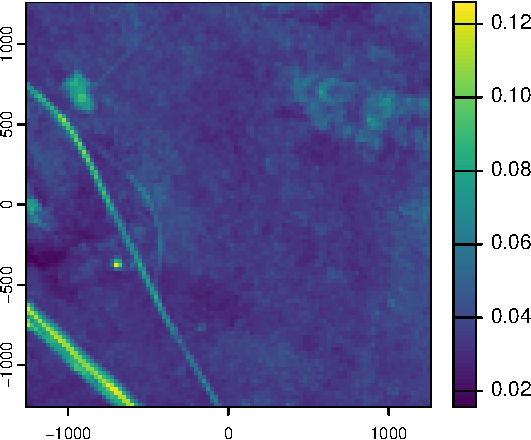
\includegraphics[keepaspectratio]{deepSSF_data_prep_S2_id_files/figure-pdf/unnamed-chunk-13-1.pdf}}

\pandocbounded{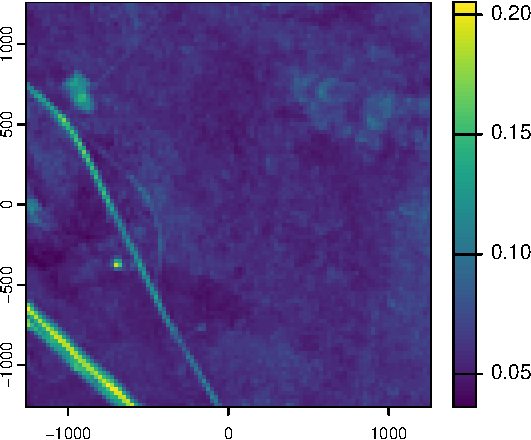
\includegraphics[keepaspectratio]{deepSSF_data_prep_S2_id_files/figure-pdf/unnamed-chunk-13-2.pdf}}

\pandocbounded{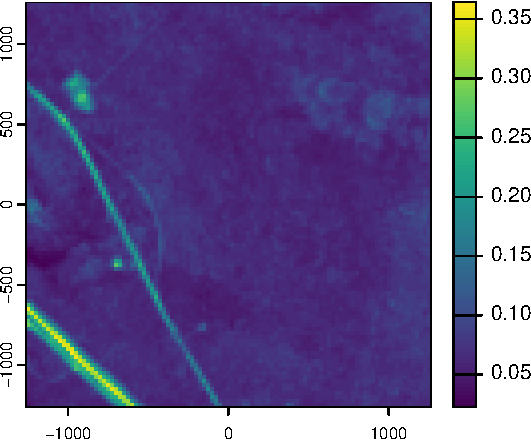
\includegraphics[keepaspectratio]{deepSSF_data_prep_S2_id_files/figure-pdf/unnamed-chunk-13-3.pdf}}

\pandocbounded{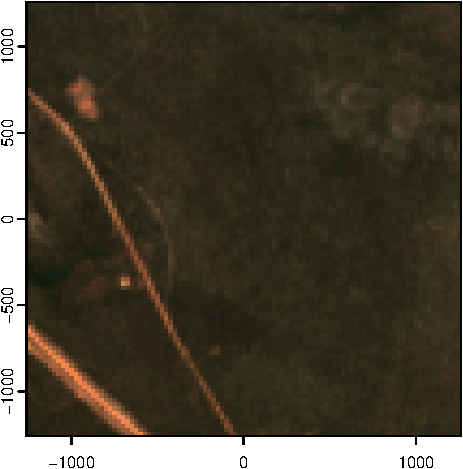
\includegraphics[keepaspectratio]{deepSSF_data_prep_S2_id_files/figure-pdf/unnamed-chunk-13-4.pdf}}

\pandocbounded{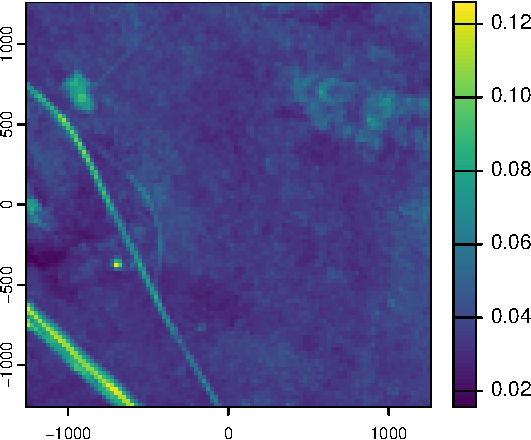
\includegraphics[keepaspectratio]{deepSSF_data_prep_S2_id_files/figure-pdf/unnamed-chunk-13-5.pdf}}

\pandocbounded{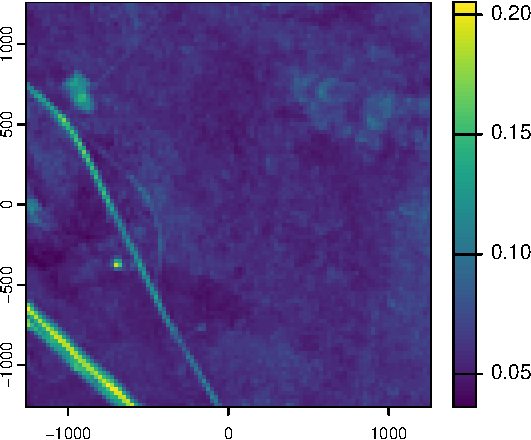
\includegraphics[keepaspectratio]{deepSSF_data_prep_S2_id_files/figure-pdf/unnamed-chunk-13-6.pdf}}

\pandocbounded{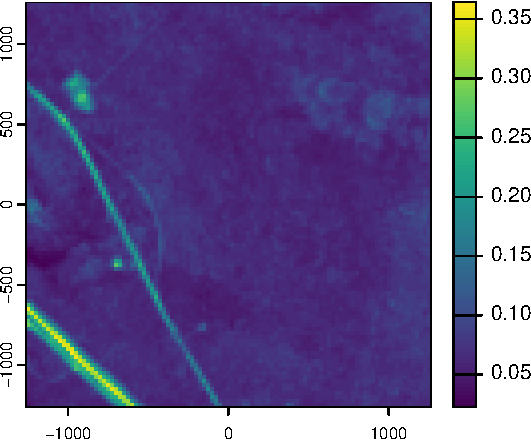
\includegraphics[keepaspectratio]{deepSSF_data_prep_S2_id_files/figure-pdf/unnamed-chunk-13-7.pdf}}

\pandocbounded{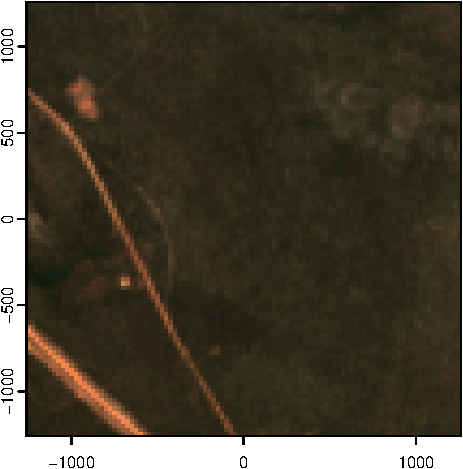
\includegraphics[keepaspectratio]{deepSSF_data_prep_S2_id_files/figure-pdf/unnamed-chunk-13-8.pdf}}

\pandocbounded{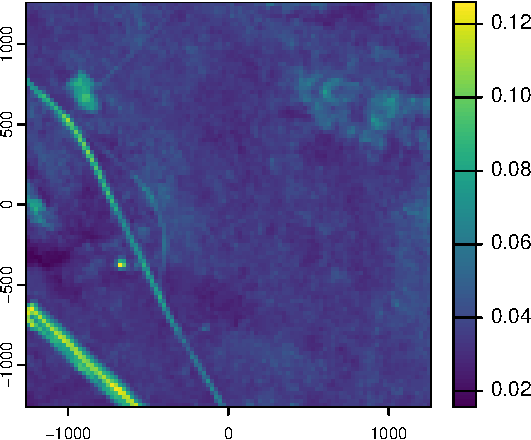
\includegraphics[keepaspectratio]{deepSSF_data_prep_S2_id_files/figure-pdf/unnamed-chunk-13-9.pdf}}

\pandocbounded{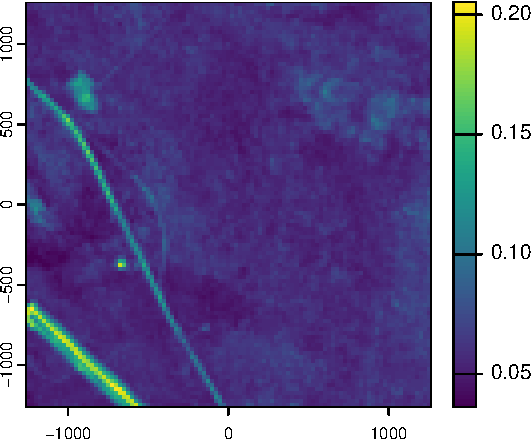
\includegraphics[keepaspectratio]{deepSSF_data_prep_S2_id_files/figure-pdf/unnamed-chunk-13-10.pdf}}

\pandocbounded{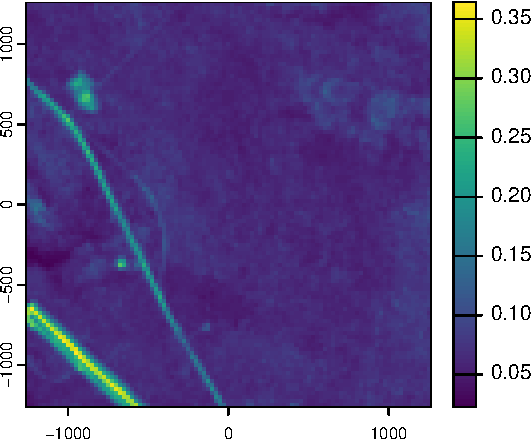
\includegraphics[keepaspectratio]{deepSSF_data_prep_S2_id_files/figure-pdf/unnamed-chunk-13-11.pdf}}

\pandocbounded{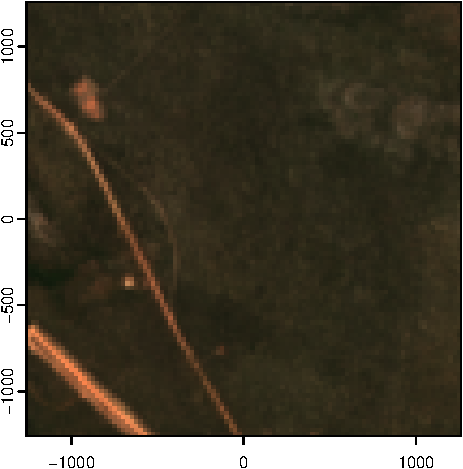
\includegraphics[keepaspectratio]{deepSSF_data_prep_S2_id_files/figure-pdf/unnamed-chunk-13-12.pdf}}

\pandocbounded{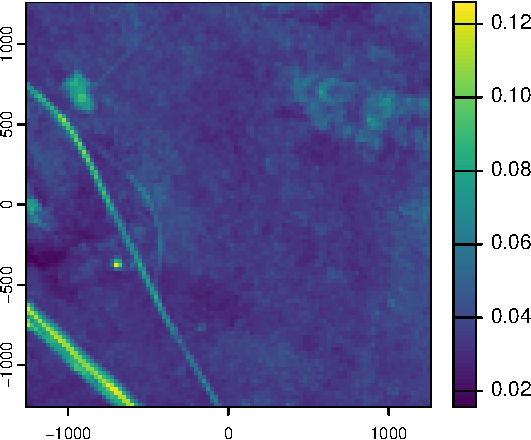
\includegraphics[keepaspectratio]{deepSSF_data_prep_S2_id_files/figure-pdf/unnamed-chunk-13-13.pdf}}

\pandocbounded{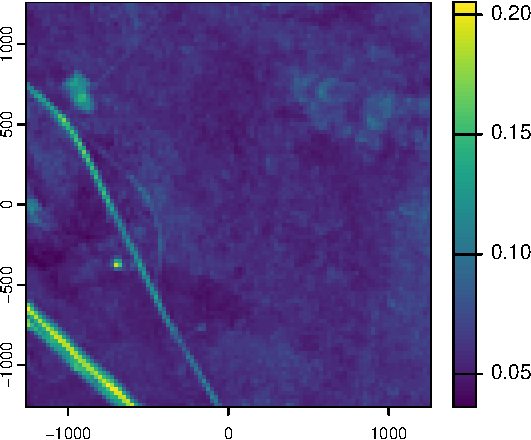
\includegraphics[keepaspectratio]{deepSSF_data_prep_S2_id_files/figure-pdf/unnamed-chunk-13-14.pdf}}

\pandocbounded{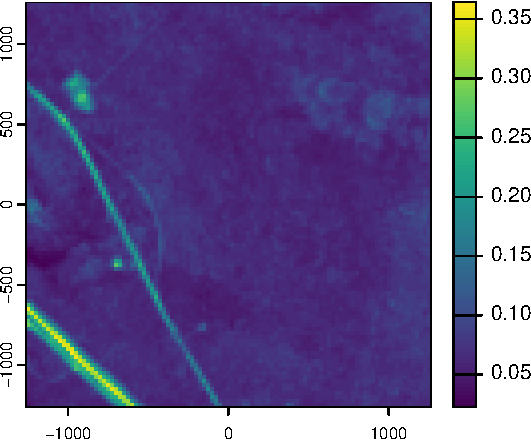
\includegraphics[keepaspectratio]{deepSSF_data_prep_S2_id_files/figure-pdf/unnamed-chunk-13-15.pdf}}

\pandocbounded{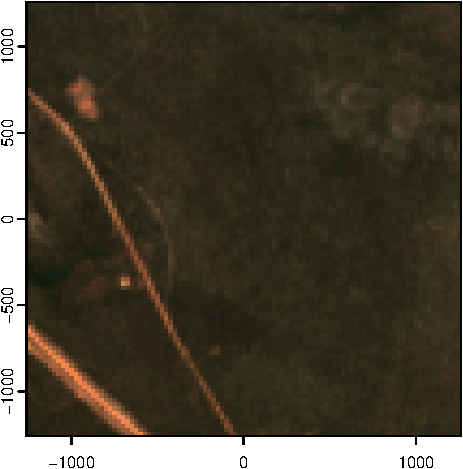
\includegraphics[keepaspectratio]{deepSSF_data_prep_S2_id_files/figure-pdf/unnamed-chunk-13-16.pdf}}

\pandocbounded{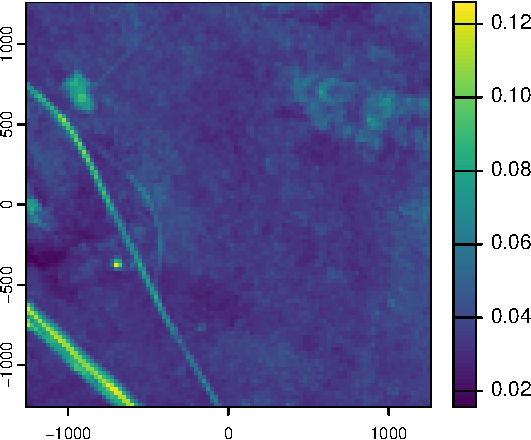
\includegraphics[keepaspectratio]{deepSSF_data_prep_S2_id_files/figure-pdf/unnamed-chunk-13-17.pdf}}

\pandocbounded{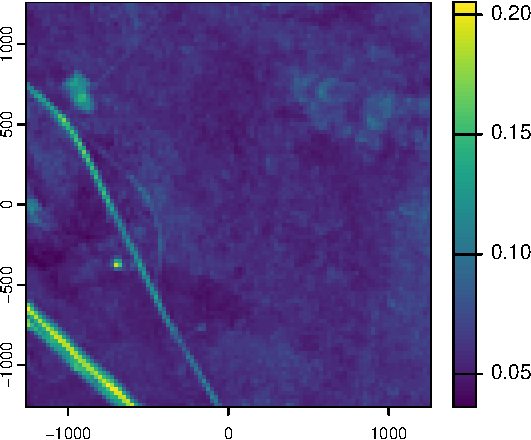
\includegraphics[keepaspectratio]{deepSSF_data_prep_S2_id_files/figure-pdf/unnamed-chunk-13-18.pdf}}

\pandocbounded{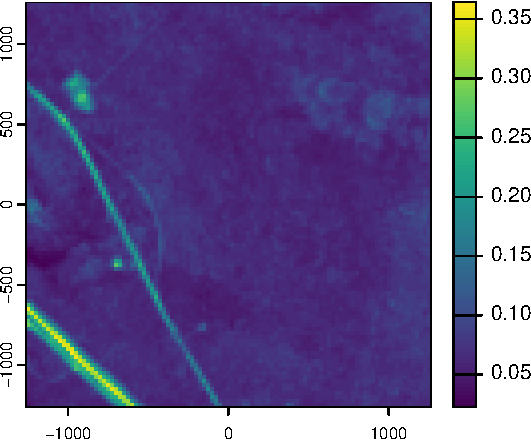
\includegraphics[keepaspectratio]{deepSSF_data_prep_S2_id_files/figure-pdf/unnamed-chunk-13-19.pdf}}

\pandocbounded{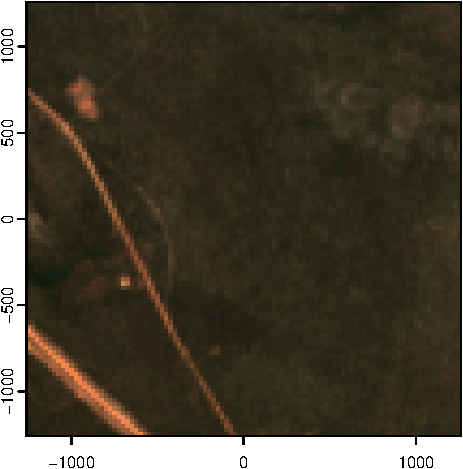
\includegraphics[keepaspectratio]{deepSSF_data_prep_S2_id_files/figure-pdf/unnamed-chunk-13-20.pdf}}




\end{document}
